\setchapterstyle{kao}
\setchapterpreamble[u]{\margintoc}
\chapter{Introduction}
\labch{intro}
\begin{fquote}[Douglas Adams][The Restaurant at the End of the Universe][1980] In the beginning the Universe was created. This has made a lot of people very angry and been widely regarded as a bad move. 
\end{fquote}

Neutrino astronomy is the youngest branch of the oldest scientific discipline. Understanding the stars has long been of central importance to society, and indeed guided exploration and scientific development of the human race for many millennia. While the centrality of astronomy as a tool for navigation has long past, it continues to be a key driver of the most human of pursuits, the expansion of our understanding of the universe in which we live. The field of astroparticle physics is grounded in recognition of the fact the capacity for human understanding ultimately surpasses even our ability to create. While terrestrial accelerators such as the Large Hadron Collider  at CERN may be capable to probing accelerating particles to $\sim 10$  TeV (the energy of a ), studies of cosmic rays in the past century have revealed that the universe  can accelerate particles to $\sim 10$  EeV, one billion times higher. If we wish to study physics at these energies, competing with nature is not a viable option. Instead, we must learn to understand the dataset that nature provides for us.

\begin{marginfigure}
	\centering 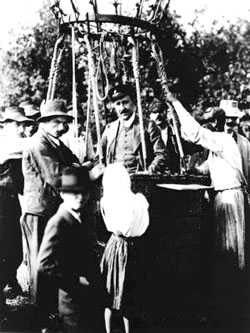
\includegraphics{intro/V-Hess-web_2.jpg}
	\caption{Victor Hess with his famous balloon, 1912.}
\end{marginfigure}

The field of \emph{astroparticle physics}, particle physics with cosmic accelerators, has been a fruitful source of mysteries in recent years. The existence of high-energy charged particles \emph{cosmic rays} was first demonstrated by Victor Hess in 1912, but their origin remains unknown over a century later. In that century, the ghostly neutrino particle was first proposed by Pauli in 192n, its existence was confirmed by in Y, its centrality in solar fusion was first posited by N, the solar neutrino flux was then measured in Z with at an unexpectedly-low rate (the so-called \emph{solar neutrino problem}), which then led to the first discovery of physics outside the Standard Model of particle physics, namely \emph{neutrino oscillations}. Experiments studying these solar neutrinos also accidentally provided us with the first case of observational astronomy with multiple 'messengers' (the observation of nearby supernova SN1987a with both neutrinos and photons), followed by the discovery of extra-terrestrial high-energy \emph{astrophyiscal neutrinos} with the IceCube detector in 2013 produced by the very same cosmic accelerators responsible for cosmic rays. A scramble to find the origin of these neutrinos led to the birth of a new field, \emph{neutrino astronomy}. The long-awaited discovery of Gravitational Waves by LIGO in 2015 was shortly thereafter followed by the discovery of a Binary Neutrino Star merger (GW170817) detected simultaneously with both photons and gravitational waves, kick-starting \emph{gravitational-wave astronomy}. One month later, the observation of a high-energy neutrino IC170922A from the direction of a flaring galactic nucleus led to the identification of the first likely source of high-energy neutrinos, TXS 0506+056. Thirty years after SN1987A, the year 2017 truly marked the dawn of an era of \emph{multi-messenger astronomy}. 

This thesis presents research probing the intersect of these new branches of astronomy with multiple messengers, incorporating searches for sources of neutrinos and gravitational waves using photons, and searches for photon sources using neutrinos. At its core, it seeks to understand what can be learned through combining knowledge from these new branches of astronomy with that of the oldest, namely photon astronomy as observed optical telescopes. The latter field is undergoing a revolution of its own, at the brink of transition from a mature human-driven field characterised by  of to an algorithm-driven one dominated by enormous data volumes. Optical astronomy is moving from object-centric to population-centric science, with scales at which detailed study of individual objects is becoming infeasible. In all three fields, a focus on rapid automated responses seeks to remove human-dependent latency in observational decisions, so-called \emph{realtime astronomy}. This drive was central in the identification of both GW170817 and TXS 0506+056, and forms a central part of this work.

This thesis begins with an introduction to ...



